% !TEX root = ../../../main.tex
% 来源：中学数学实验教材·第一册（代数）
% 章节：因式分解与余式定理 / 辗转相除法
% 原始文件：5.tex，行 2859-2874
% 类型：tikz
% ---
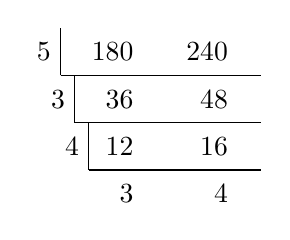
\begin{tikzpicture}[scale=.6]
\foreach \y/\ytext in {0/3, 1/12,2/36,3/180}
{
    \node at (0, \y)[left]{\ytext};
}
\foreach \y/\ytext in {0/4, 1/16,2/48,3/240}
{
    \node at (2, \y)[left]{\ytext};
}
\foreach \y/\x in {.5/4,1.5/3,2.5/5}
{
    \draw (-1-\y*0.3,\y)--(2.5,\y);
    \draw (-1-\y*.3,\y)--node[left]{\x}(-1-\y*.3,\y+1);
}

\end{tikzpicture}
